\section{Introduction}

Deep neural networks have been successfully applied to various natural language processing tasks.
%where end-to-end training become a primary option.
As the design of neural networks evolves, there is a trend of increasing model complexity become clear in terms of both the architecture and the parameter count. 
%
Although expressive models help improve the prediction performance, the fundamental lack of interpretability leads many researchers to consider neural network models black boxes. 
%
The ability to interpret model internals and reason about predictions is essential for understanding the limitation of the models and improving upon them.

%Without understanding the background meaning that features carry, visualization relies
%on proper quantification analysis (cite). Such analysis is not easy to come up with,
%and is tied to specific task (cite).

Recently, the attention networks have recently become  widely-adopted~\cite{bahdanau2014neural,seo2016bidirectional,Parikh2016, VaswaniShazeerParmar2017}. Attention not only improves the model performance but also yields interpretable intermediate representations (i.e., alignment among words). As a result, attention can provide a natural interface for analyzing the internals of neural networks. Conducting analysis directly on the raw attention values can be challenging for human users, and therefore, visual representations that highlight word alignments between sentences have been proposed, such as the bipartite graph and the heatmap of the attention matrix \cite{LiChenHovy2015, li2016understanding, lee2017interactive}.  However, many challenges remain. Firstly, for some NLP tasks, the word sequences pair for which the attention is computed can be highly asymmetrical (i.e., in machine comprehension, the context paragraph can be much longer than the question sentence), which the standard visual encoding cannot adequately handle.  Also, many previous works present the attention in a static setting. However, the ability to provide an interactive environment in which the user can instantaneously look at how changes in the input affect the attention, and how small variations in the attention alter the prediction, is crucial for interpreting the model. Finally, many previous visualization efforts, despite revealing many exciting results, focus more on illustrating potentially useful visualization techniques than on providing a flexible software tool that can be easily integrated into an existing code base. As a result, applying these proposed techniques to real-world examples may involve substantial engineering effort, which could prevent wide adoption.

\begin{figure}[htbp]
\centering
\vspace{-2mm}
 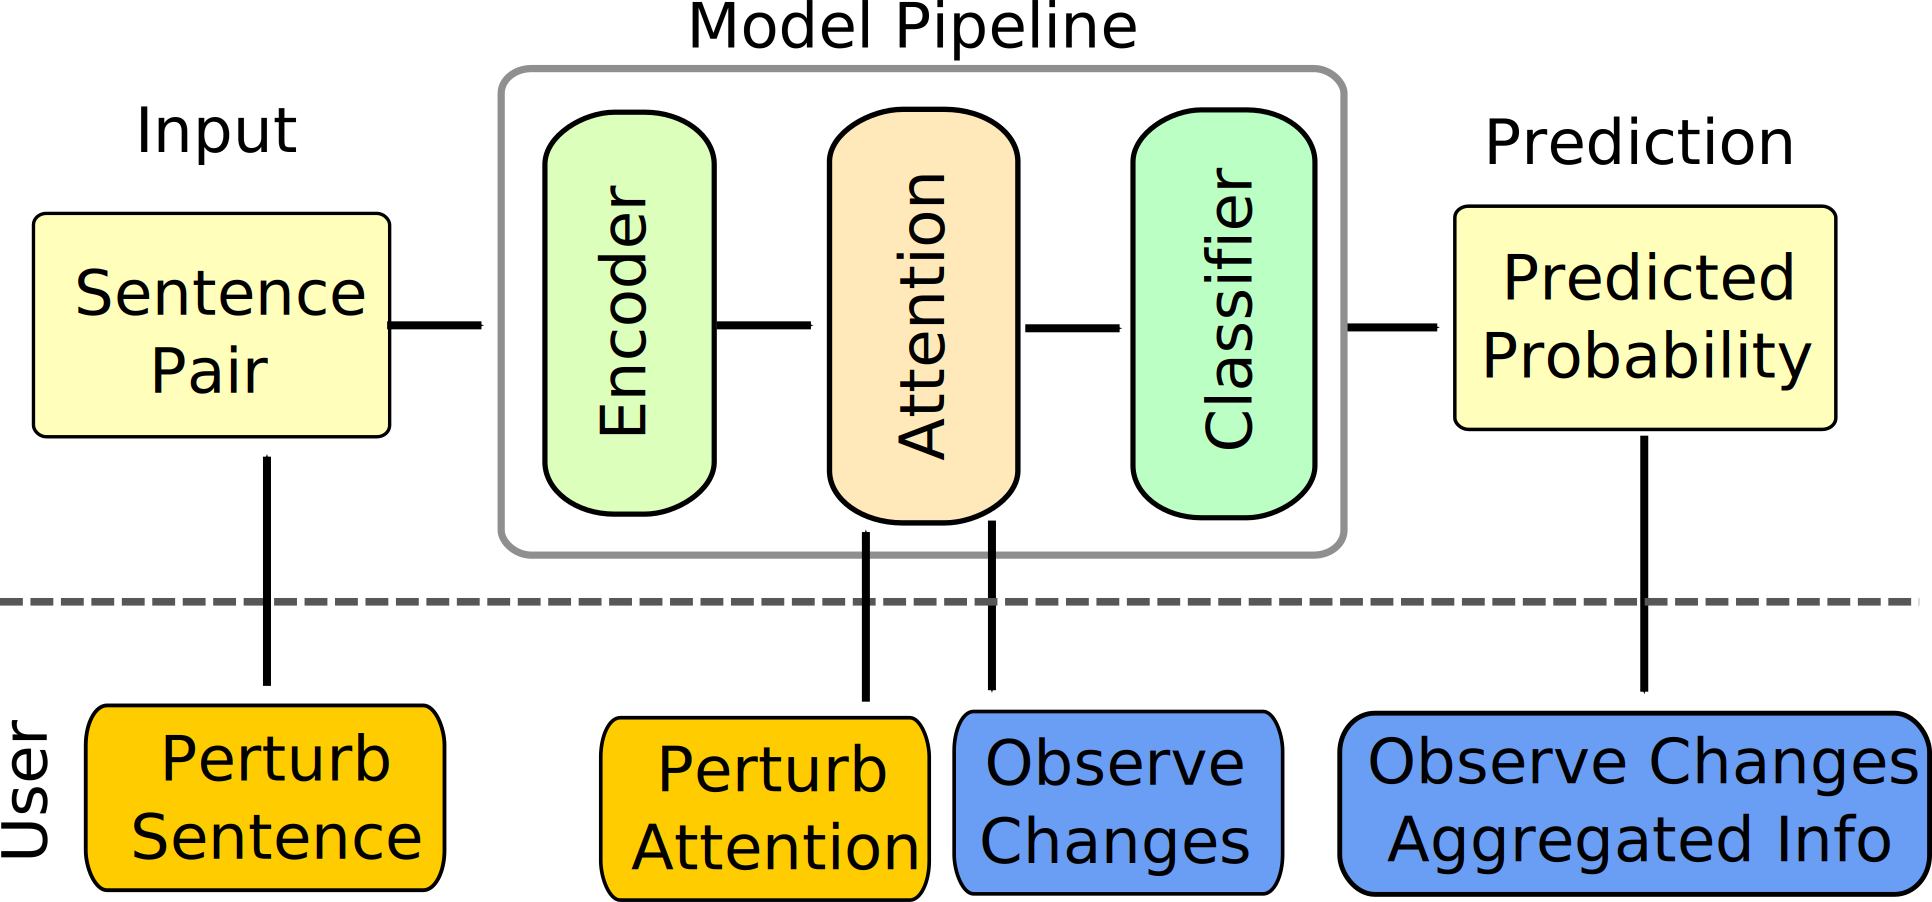
\includegraphics[width=1.0\linewidth]{pipeline}
 \vspace{-3mm}
 \caption{
 Perturbation-driven interrogation of the end-to-end models that follow the encoder, attention, and classifier structure. The user can generate a small perturbation of the input (i.e., replacing synonyms, paraphrasing), edit the attention, and observe the changes.
 }
 \vspace{-3mm}
\label{fig:modelPipeline}
\end{figure}


To address these challenges in interpreting attention-based models, 
we introduce a Python library that allows users to create web-based interactive visual analytics environments,
in which they can interrogate the model by perturbing the input text and observing the effects on the attention and prediction, or modifying the attention and studying how it affects predictions (see Figure~\ref{fig:modelPipeline}).
%
We demonstrate our library applied to two NLP tasks: natural language
inference (NLI) and machine comprehension (MC). 
%For the NLI task, we visualize
%decomposable attention networks which represents a series of strongly performing models \cite{Parikh2016}.
%For the MC task, we present your visualization methods on bidirectional attention flow model,
%which also represents a line of state-of-the-art models \cite{Seo2016}.


%In summary, our key contributions are:
%\begin{itemize}
%	\item Introduce an flexible visualization system for creating customized interactive visual analytic environment for attention centric neural networks models;
%	\item Illustrate the importance of envire
%	\item Demonstrate our system on two major NLP tasks with strong-performing
%	models. We observe functional limitations of these models which can be helpful
%	for future improvement on modeling.
%\end{itemize}


%%% Local Variables:
%%% mode: latex
%%% TeX-master: "NLPVis-demo-paper"
%%% End:
